%%%%%%%%%%%%%%%%%%%%%%%%%%%%%%%%%%%%%%%%%%%%%%%%%%%%%%%%%%%%%%%%%%%%%
% LaTeX Template: Project Titlepage Modified (v 0.1) by rcx
%
% Original Source: http://www.howtotex.com
% Date: February 2014
% 
% This is a title page template which be used for articles & reports.
% 
% This is the modified version of the original Latex template from
% aforementioned website.
% 
%%%%%%%%%%%%%%%%%%%%%%%%%%%%%%%%%%%%%%%%%%%%%%%%%%%%%%%%%%%%%%%%%%%%%%

\documentclass[12pt]{report}
\usepackage[a4paper]{geometry}
\usepackage[myheadings]{fullpage}
\usepackage{fancyhdr}
\usepackage{lastpage}
\usepackage{graphicx, wrapfig,setspace, booktabs}
\usepackage[T1]{fontenc}
\usepackage[font=small, labelfont=bf]{caption}
\usepackage{fourier}
\usepackage[protrusion=true, expansion=true]{microtype}
\usepackage[english]{babel}
\usepackage{sectsty}
\usepackage{lipsum}
\usepackage[hyphens]{url}
%\usepackage{subfig}
\usepackage{hyperref}
\usepackage{alphalph}
\usepackage[utf8]{inputenc}
\usepackage{multicol}
\usepackage{amsmath}
\usepackage{subfigure}
\renewcommand*{\thesubfigure}{%
\alphalph{\value{subfigure}}%
}%


\newcommand{\HRule}[1]{\rule{\linewidth}{#1}}
\onehalfspacing
\setcounter{tocdepth}{5}
\setcounter{secnumdepth}{5}
\usepackage{float}

\usepackage[backend=bibtex,style=chem-acs,biblabel=dot]{biblatex}
\addbibresource{references.bib}

%-------------------------------------------------------------------------------
% HEADER & FOOTER
%-------------------------------------------------------------------------------
\pagestyle{fancy}
\fancyhf{}
\setlength\headheight{15pt}
\fancyhead[L]{CS7015: PA4}
\fancyhead[R]{Deep Learning}
\fancyfoot[R]{Page \thepage\ of \pageref{LastPage}}
%-------------------------------------------------------------------------------
% TITLE PAGE
%-------------------------------------------------------------------------------

\begin{document}

\title{ \normalsize \textsc{CS7015 : Deep Learning}
		\\ [2.0cm]
		\HRule{0.5pt} \\
		\LARGE \textbf{\uppercase{Programming Assignment 5}}\\
        \large{- RBM -}
		\HRule{2pt} \\ [0.5cm]
		\normalsize \today \vspace*{5\baselineskip}}

\date{}

\author{
		Student ID:  \\ 
		Namida M - EE15B123 \\
		Ganga Meghanath - EE15B025
		}

\renewcommand\thesection{\arabic{section}}
\maketitle
\tableofcontents
\newpage

%-------------------------------------------------------------------------------
% Section title formatting
\sectionfont{\scshape}
%-------------------------------------------------------------------------------

%-------------------------------------------------------------------------------
% BODY
%-------------------------------------------------------------------------------

\section{Introduction}
RBMs can be used to learn hidden representations (h) from the raw features (V ). The objective of the assignment is to train RBMs using the Contrastive Divergence (CD) algorithm. The training data used is Fashion MNIST. The 784 dimensional (V) dataset is thresholded into binary data (using a threshold of 127) to learn a n-dimensional hidden representation (h).
%-------------------------------------------------------------------------------
%DATA ANALYSIS
%-------------------------------------------------------------------------------

\section{t-SNE Plots}

\begin{table}[H]
  \centering
  \begin{tabular}{ | c | c | c | c || c | c | c| c |}
    \hline
    \textbf{lr} & \textbf{n} & \textbf{k} & \textbf{t-SNE} & \textbf{lr} & \textbf{n} & \textbf{k} & \textbf{t-SNE} \\
     &  &  &  & & & & \\ \hline
    1e-3 & 256 & 1 &
    \begin{minipage}{.3\textwidth}
      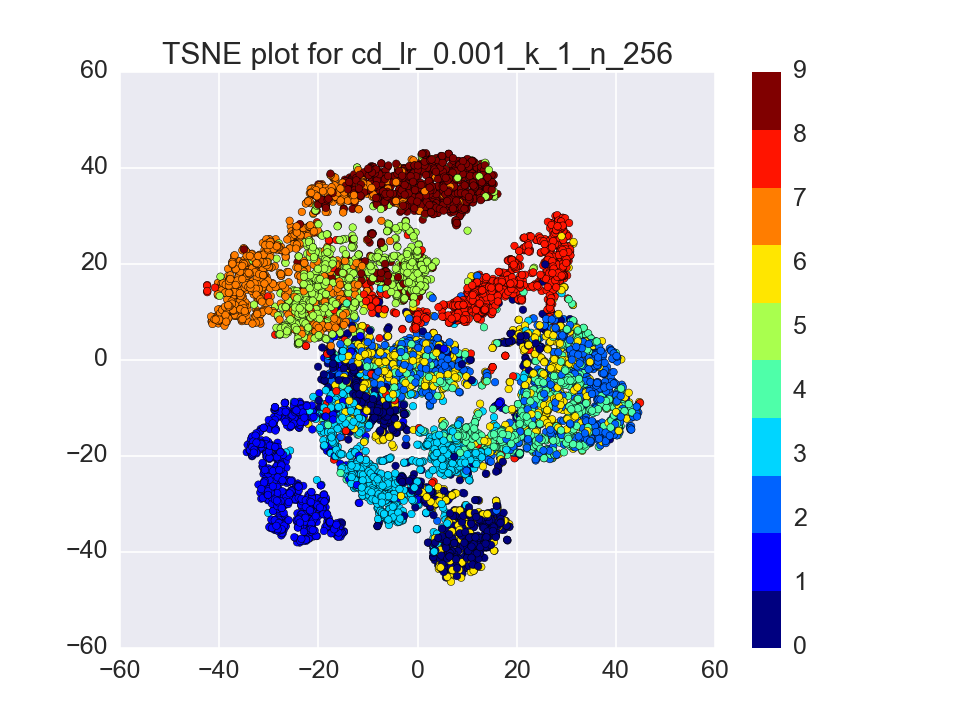
\includegraphics[scale=0.25]{cd_lr_0_001_k_1_n_256.png}
    \end{minipage}
	&
    1e-3 & 128 & 1 &
    \begin{minipage}{.3\textwidth}
      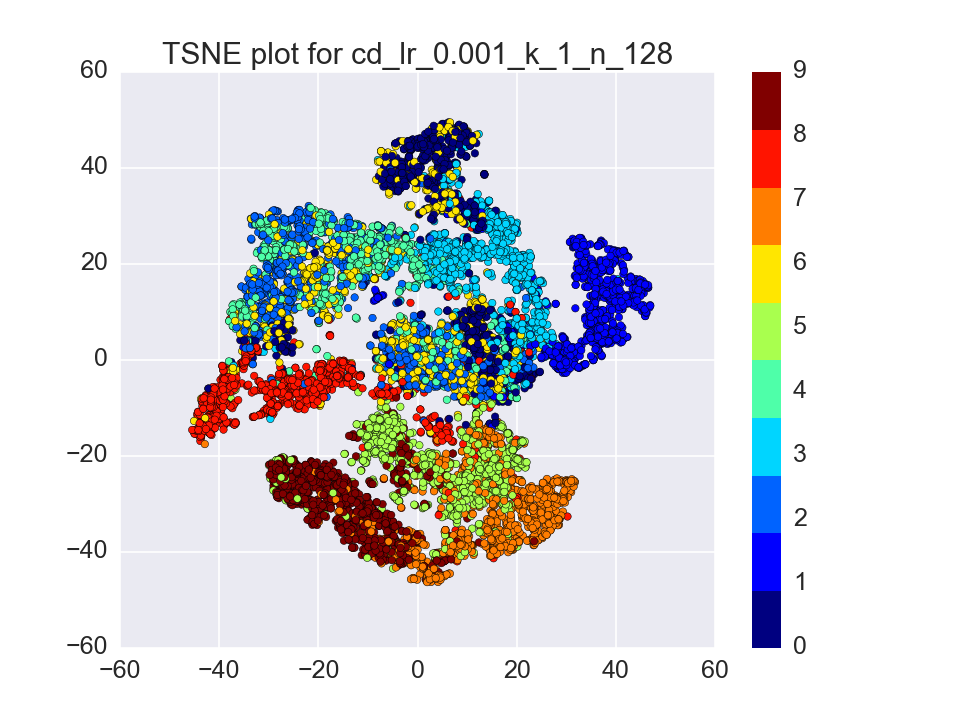
\includegraphics[scale=0.25]{cd_lr_0_001_k_1_n_128.png}
      %\includegraphics[width=\linewidth, height=60mm]{tiger}
    \end{minipage}
    \\ \hline
    1e-3 & 256 & 2 &
    \begin{minipage}{.3\textwidth}
      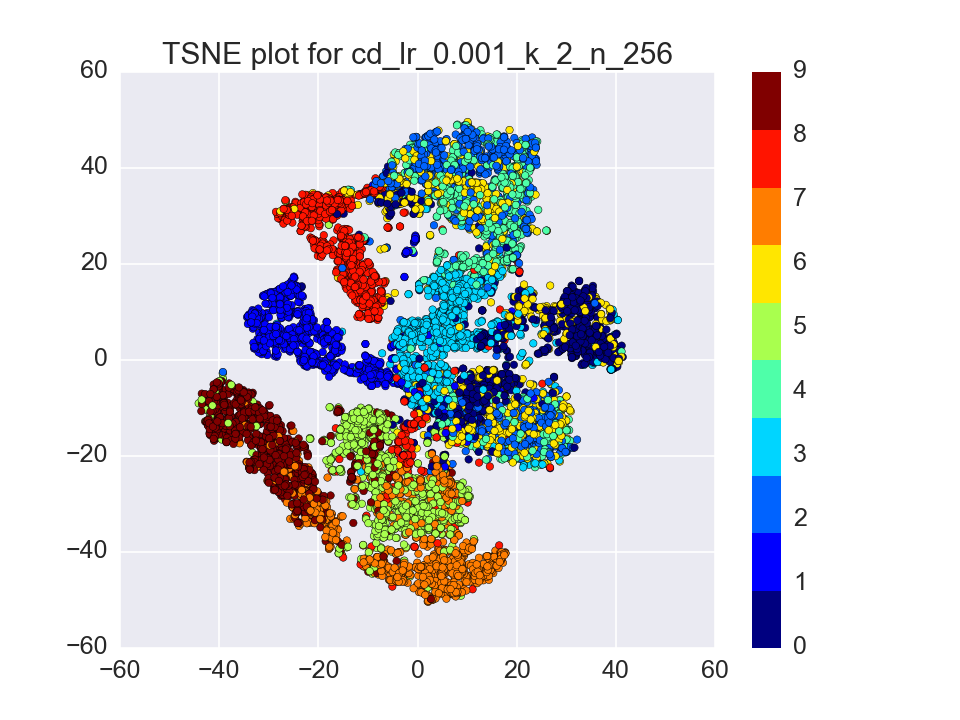
\includegraphics[scale=0.25]{cd_lr_0_001_k_2_n_256.png}
      %\includegraphics[width=\linewidth, height=60mm]{tiger}
    \end{minipage}
    & 1e-3 & 128 & 2 &
    \begin{minipage}{.3\textwidth}
      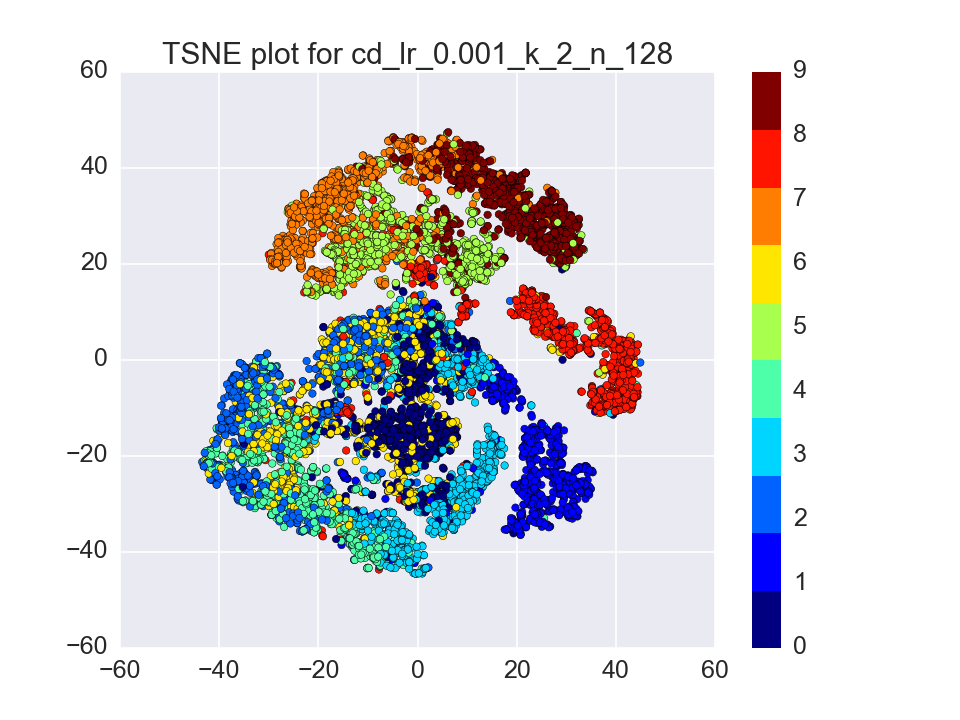
\includegraphics[scale=0.25]{cd_lr_0_001_k_2_n_128.png}
      %\includegraphics[width=\linewidth, height=60mm]{tiger}
    \end{minipage}
    \\ \hline
    1e-3 & 256 & 4 &
    \begin{minipage}{.3\textwidth}
      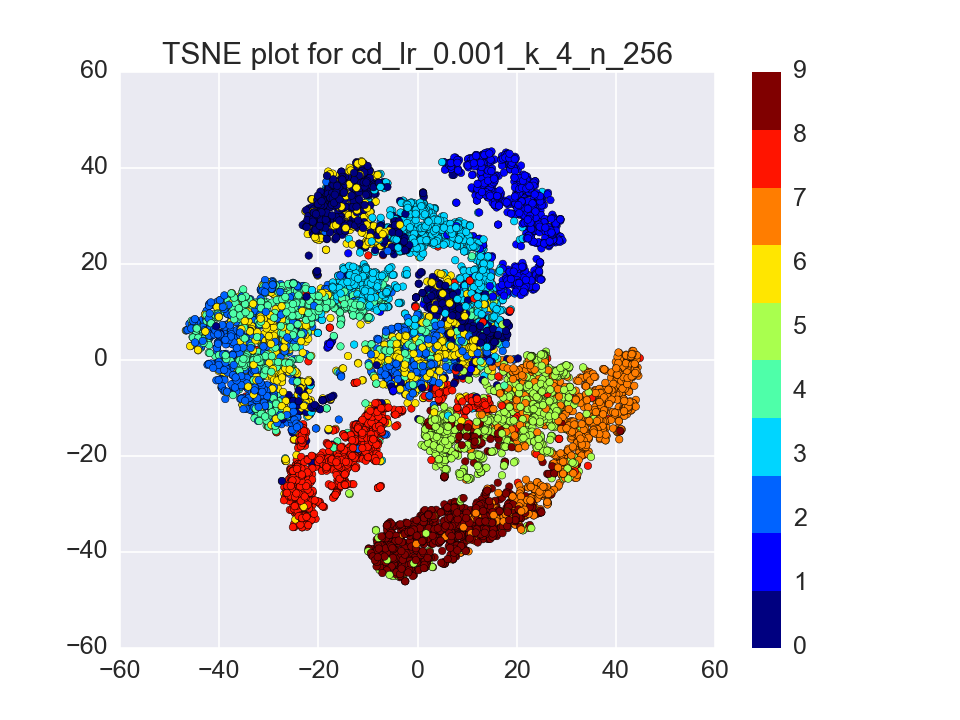
\includegraphics[scale=0.25]{cd_lr_0_001_k_4_n_256.png}
      %\includegraphics[width=\linewidth, height=60mm]{tiger}
    \end{minipage}
     & 1e-3 & 128 & 4 &
    \begin{minipage}{.3\textwidth}
      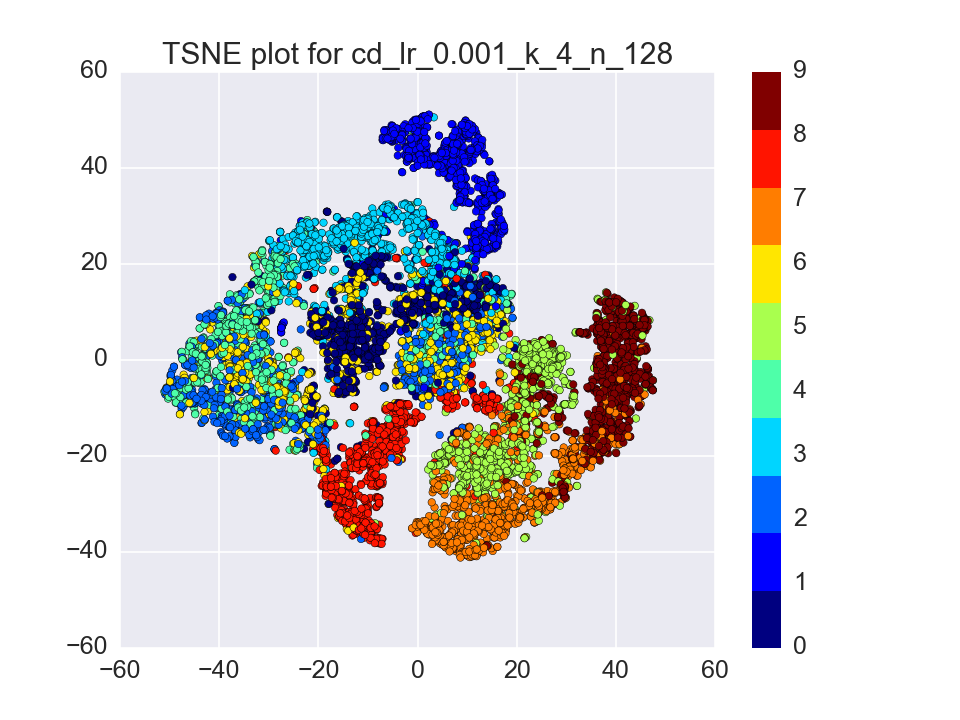
\includegraphics[scale=0.25]{cd_lr_0_001_k_4_n_128.png}
      %\includegraphics[width=\linewidth, height=60mm]{tiger}
    \end{minipage}
    \\ \hline
    1e-3 & 256 & 8 &
    \begin{minipage}{.3\textwidth}
      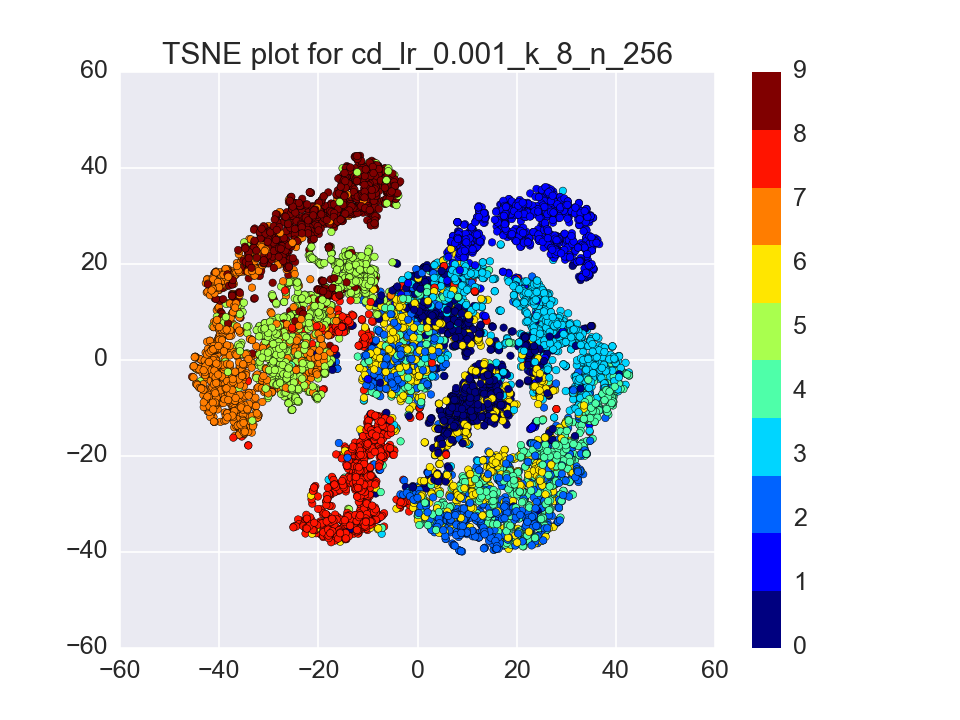
\includegraphics[scale=0.25]{cd_lr_0_001_k_8_n_256.png}
      %\includegraphics[width=\linewidth, height=60mm]{tiger}
    \end{minipage}
     & 1e-3 & 128 & 8 &
    \begin{minipage}{.3\textwidth}
      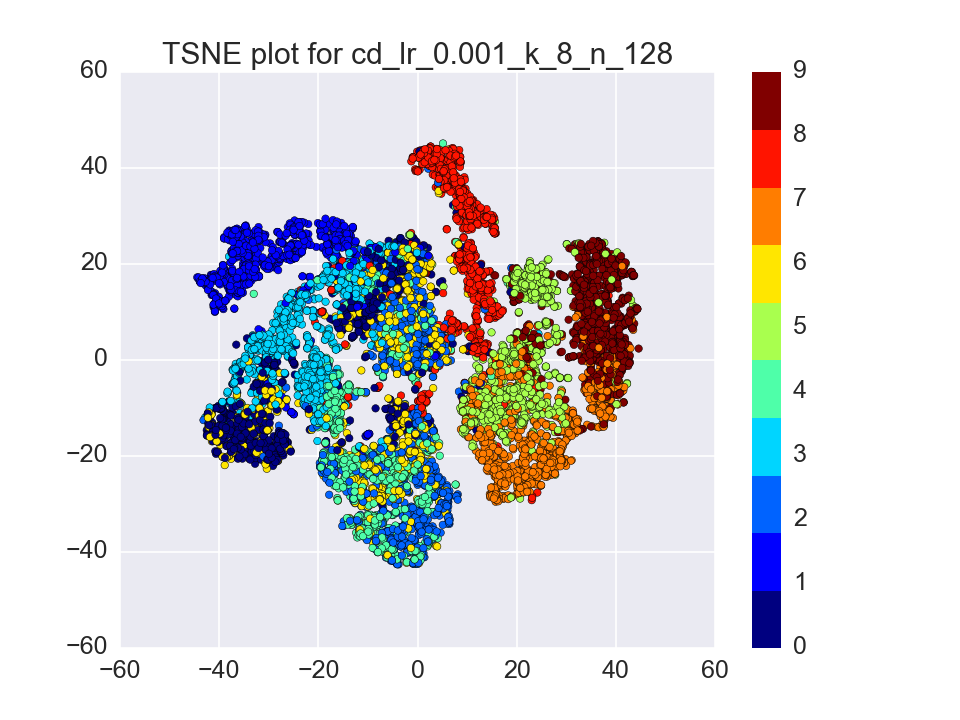
\includegraphics[scale=0.25]{cd_lr_0_001_k_8_n_128.png}
      %\includegraphics[width=\linewidth, height=60mm]{tiger}
    \end{minipage}
    \\ \hline
        1e-3 & 256 & 16 &
    \begin{minipage}{.3\textwidth}
      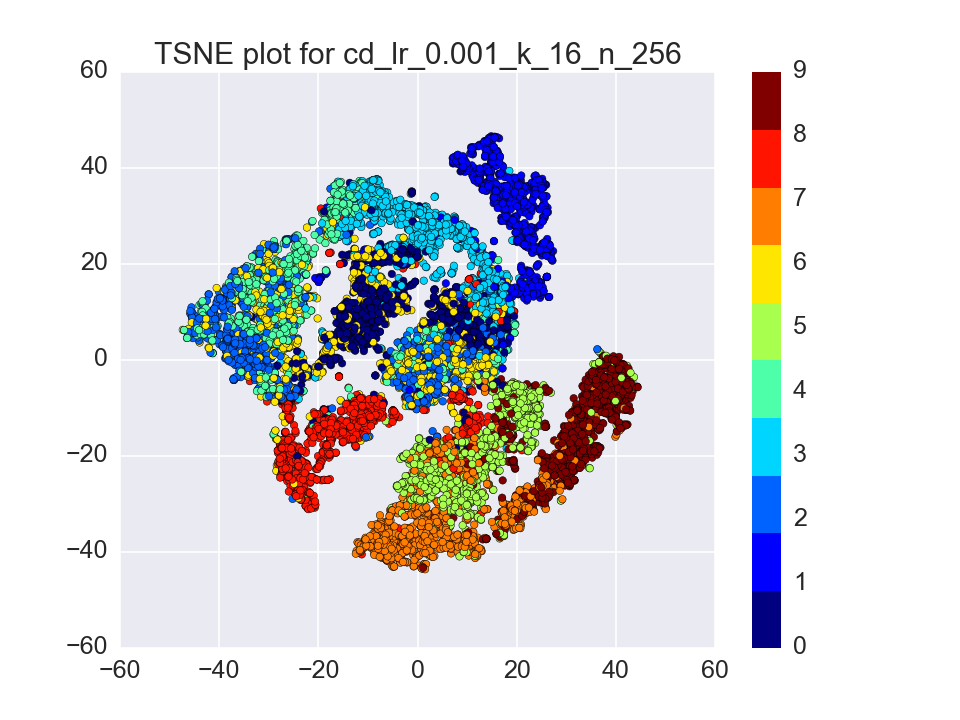
\includegraphics[scale=0.25]{cd_lr_0_001_k_16_n_256.png}
      %\includegraphics[width=\linewidth, height=60mm]{tiger}
    \end{minipage}
     & 1e-3 & 128 & 16 &
    \begin{minipage}{.3\textwidth}
      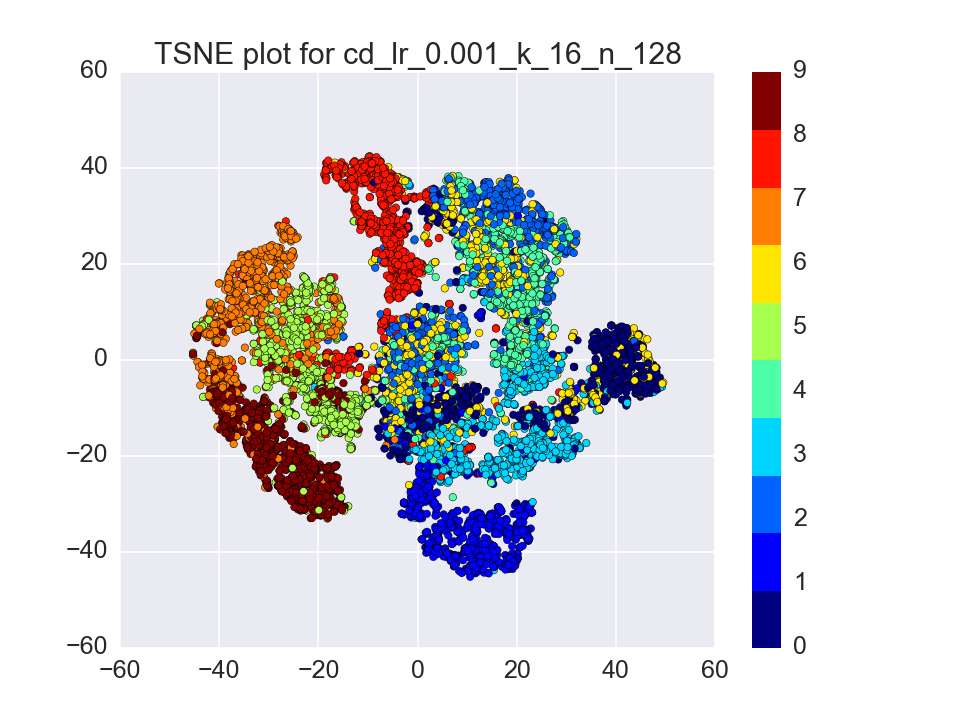
\includegraphics[scale=0.25]{cd_lr_0_001_k_16_n_128.png}
      %\includegraphics[width=\linewidth, height=60mm]{tiger}
    \end{minipage}
    \\ \hline
        1e-3 & 256 & 32 &
    \begin{minipage}{.3\textwidth}
      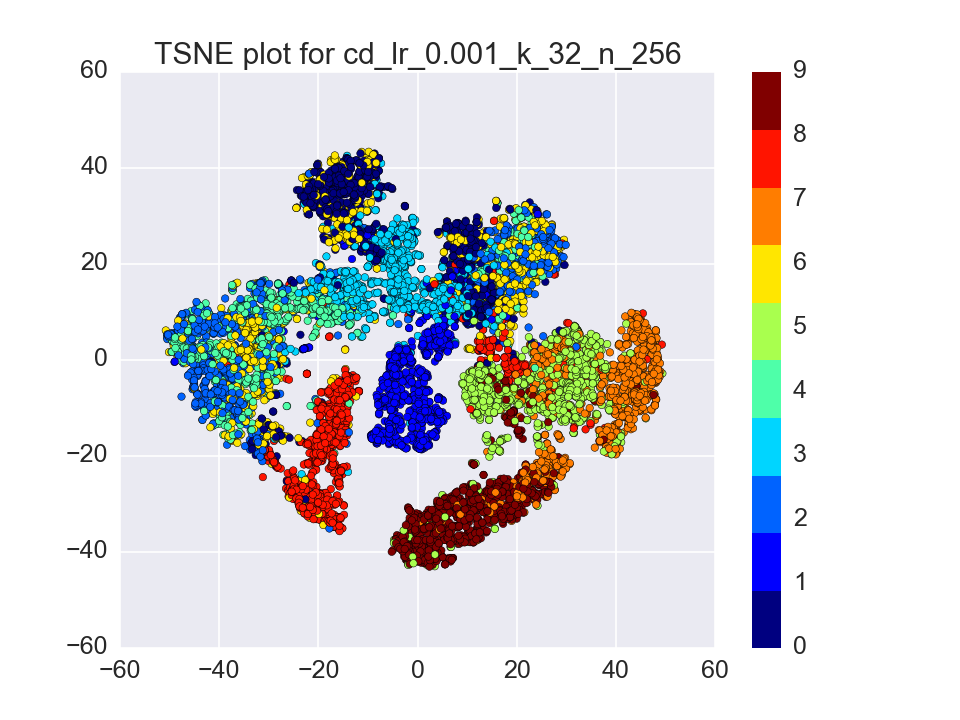
\includegraphics[scale=0.25]{cd_lr_0_001_k_32_n_256.png}
      %\includegraphics[width=\linewidth, height=60mm]{tiger}
    \end{minipage}
     & 1e-3 & 128 & 32 &
    \begin{minipage}{.3\textwidth}
      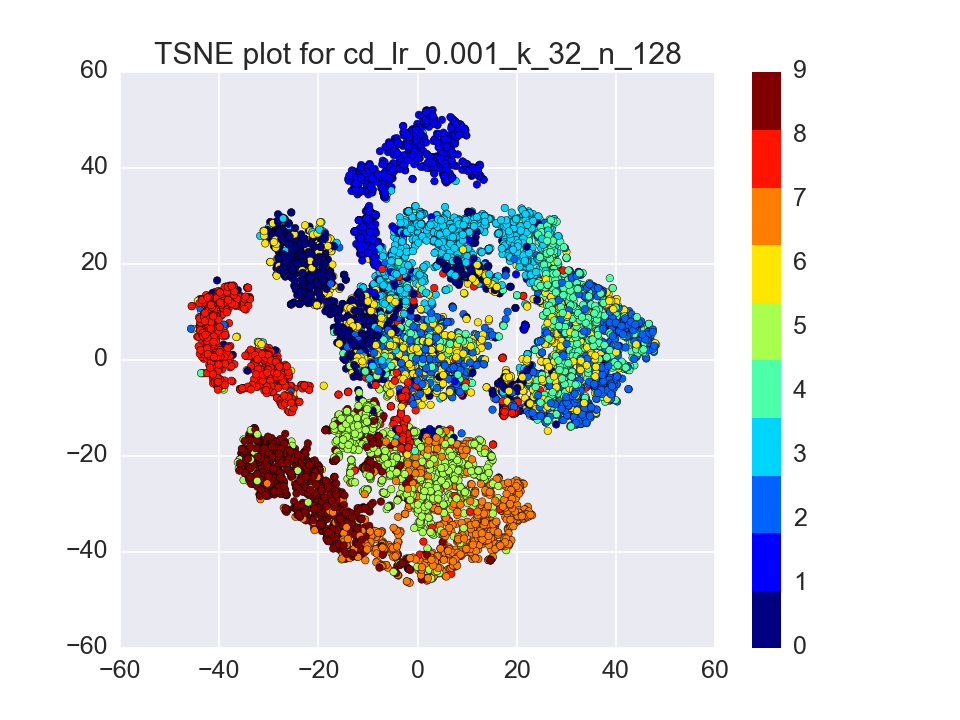
\includegraphics[scale=0.25]{cd_lr_0_001_k_32_n_128.png}
      %\includegraphics[width=\linewidth, height=60mm]{tiger}
    \end{minipage}
    \\ \hline
  \end{tabular}
\end{table}


\begin{table}[H]
  \centering
  \begin{tabular}{ | c | c | c | c || c | c | c| c |}
    \hline
    \textbf{lr} & \textbf{n} & \textbf{k} & \textbf{t-SNE} & \textbf{lr} & \textbf{n} & \textbf{k} & \textbf{t-SNE} \\
     &  &  &  & & & & \\ \hline
    1e-3 & 64 & 1 &
    \begin{minipage}{.3\textwidth}
      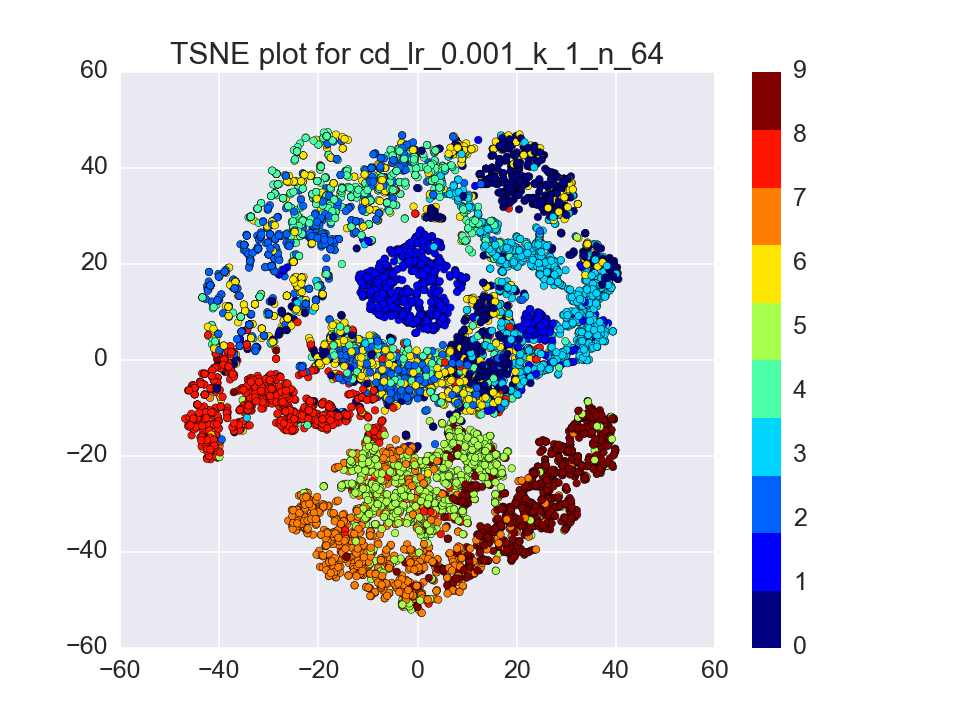
\includegraphics[scale=0.25]{cd_lr_0_001_k_1_n_64.png}
    \end{minipage}
	&
    1e-4 & 256 & 1 &
    \begin{minipage}{.3\textwidth}
      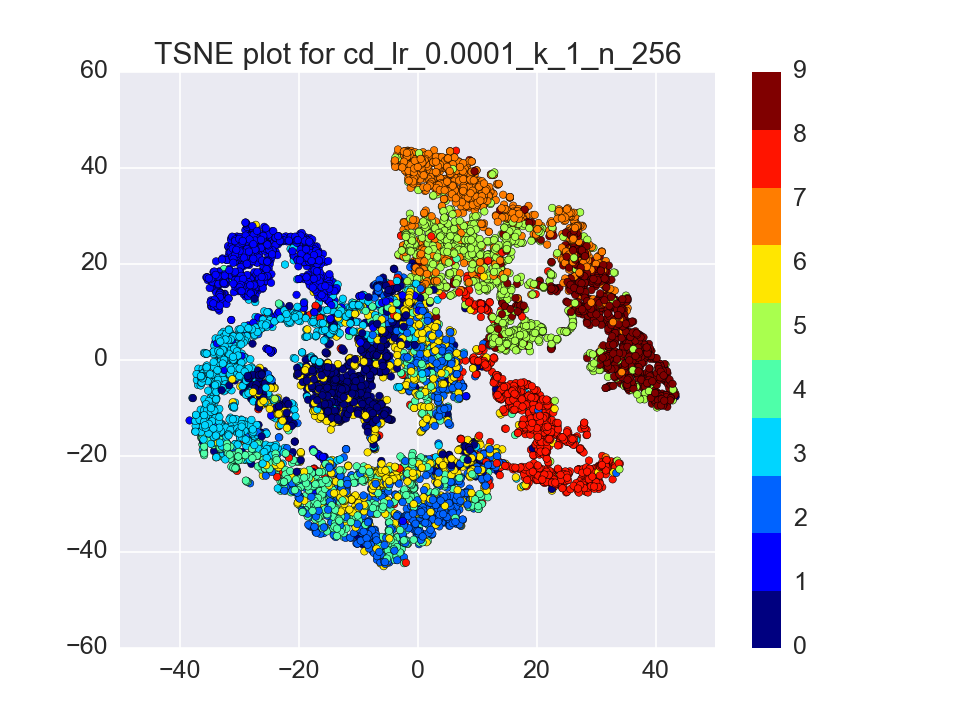
\includegraphics[scale=0.25]{cd_lr_0_0001_k_1_n_256.png}
      %\includegraphics[width=\linewidth, height=60mm]{tiger}
    \end{minipage}
    \\ \hline
    1e-3 & 64 & 2 &
    \begin{minipage}{.3\textwidth}
      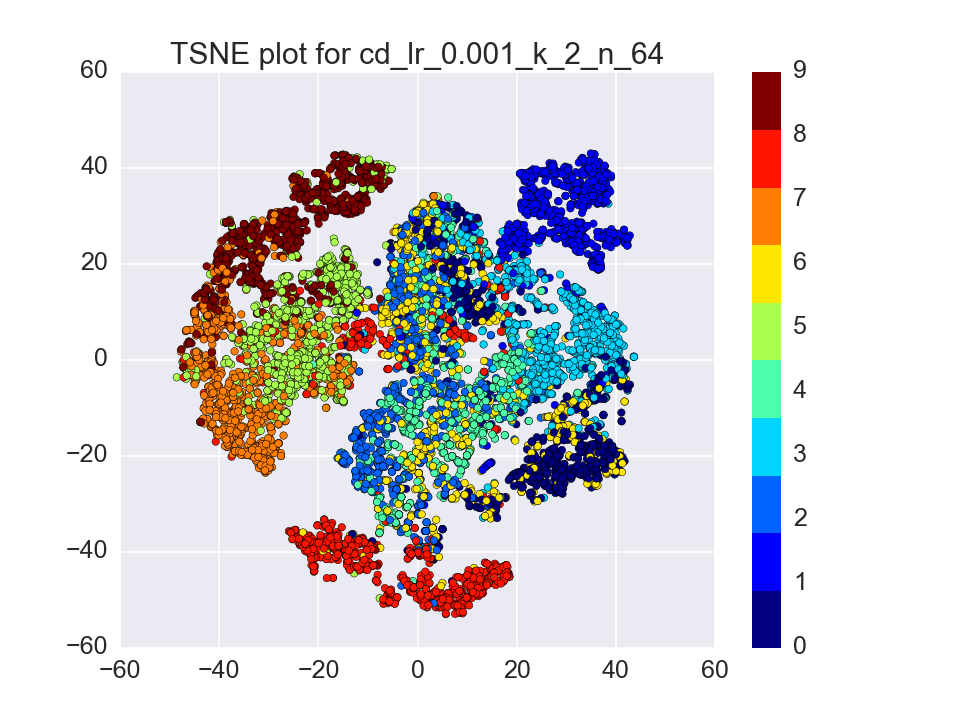
\includegraphics[scale=0.25]{cd_lr_0_001_k_2_n_64.png}
    \end{minipage}
	&
    1e-4 & 256 & 2 &
    \begin{minipage}{.3\textwidth}
      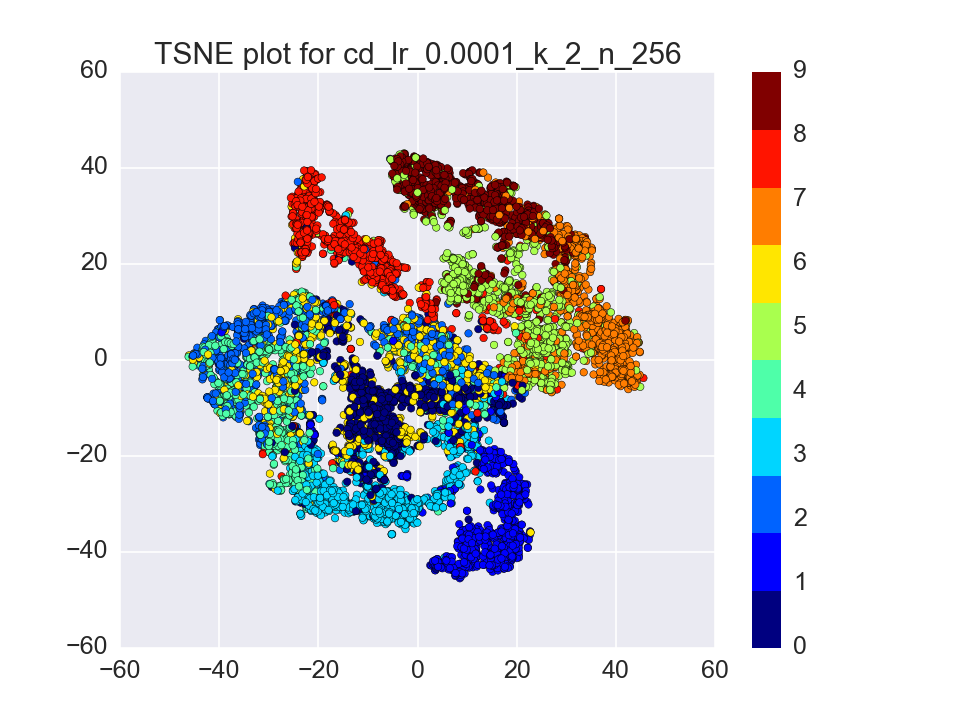
\includegraphics[scale=0.25]{cd_lr_0_0001_k_2_n_256.png}
      %\includegraphics[width=\linewidth, height=60mm]{tiger}
    \end{minipage}
    \\ \hline
     1e-3 & 64 & 4 &
    \begin{minipage}{.3\textwidth}
      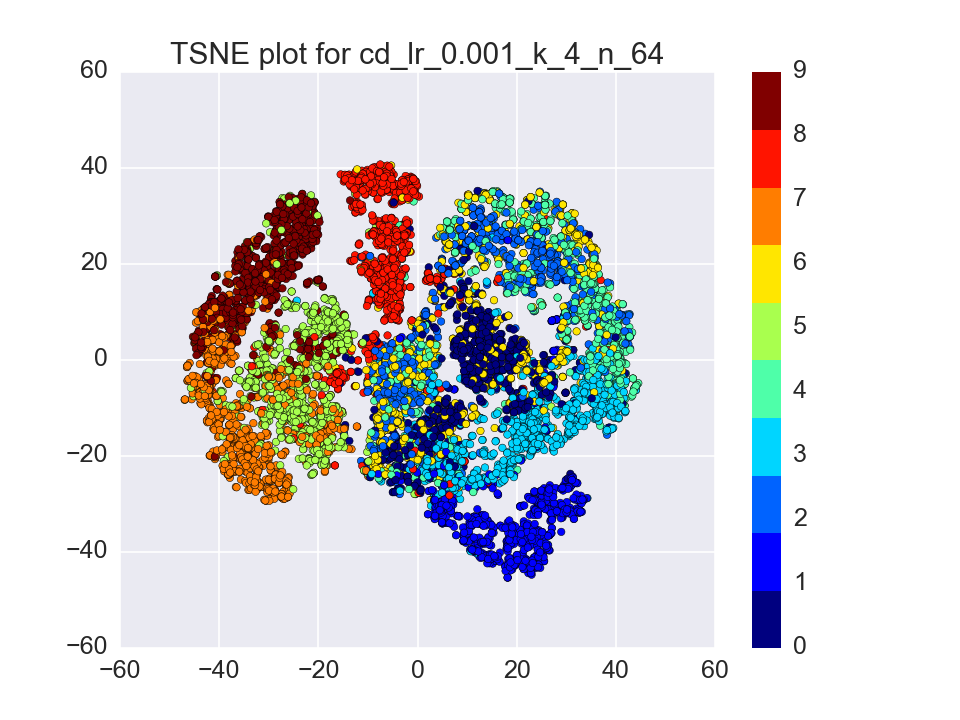
\includegraphics[scale=0.25]{cd_lr_0_001_k_4_n_64.png}
    \end{minipage}
	&
    1e-4 & 256 & 4 &
    \begin{minipage}{.3\textwidth}
      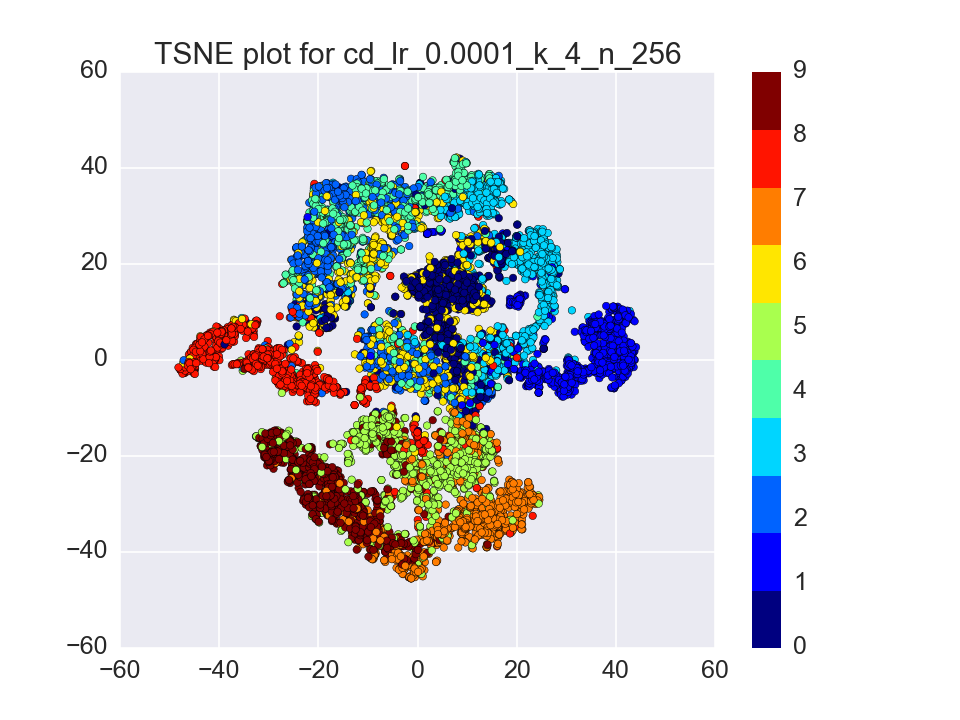
\includegraphics[scale=0.25]{cd_lr_0_0001_k_4_n_256.png}
      %\includegraphics[width=\linewidth, height=60mm]{tiger}
    \end{minipage}
    \\ \hline
    1e-3 & 64 & 8 &
    \begin{minipage}{.3\textwidth}
      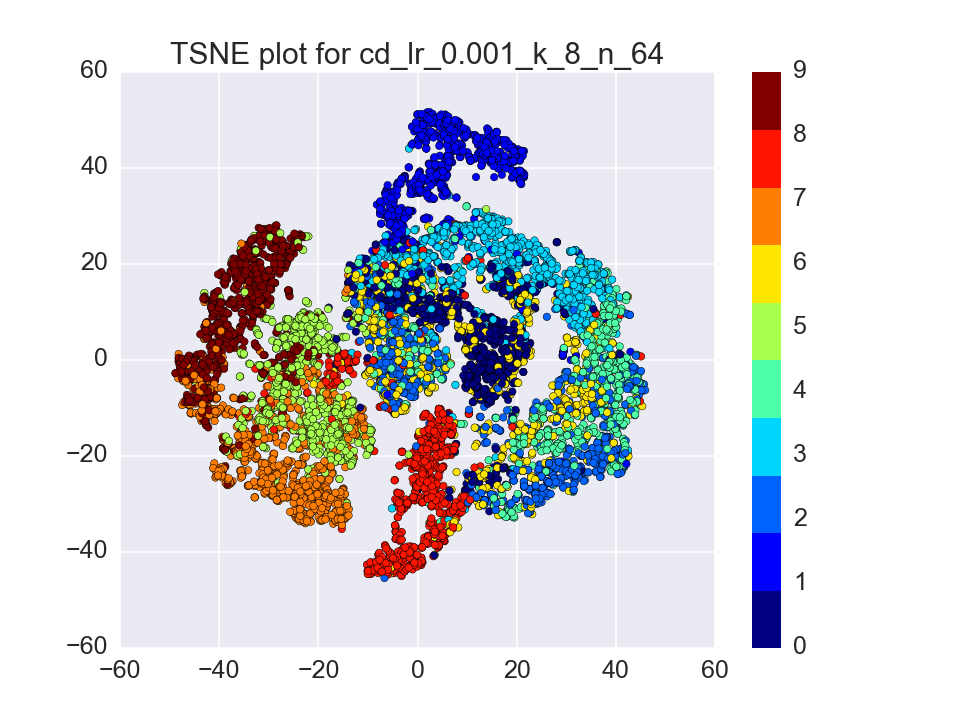
\includegraphics[scale=0.25]{cd_lr_0_001_k_8_n_64.png}
    \end{minipage}
	&
    1e-4 & 256 & 8 &
    \begin{minipage}{.3\textwidth}
      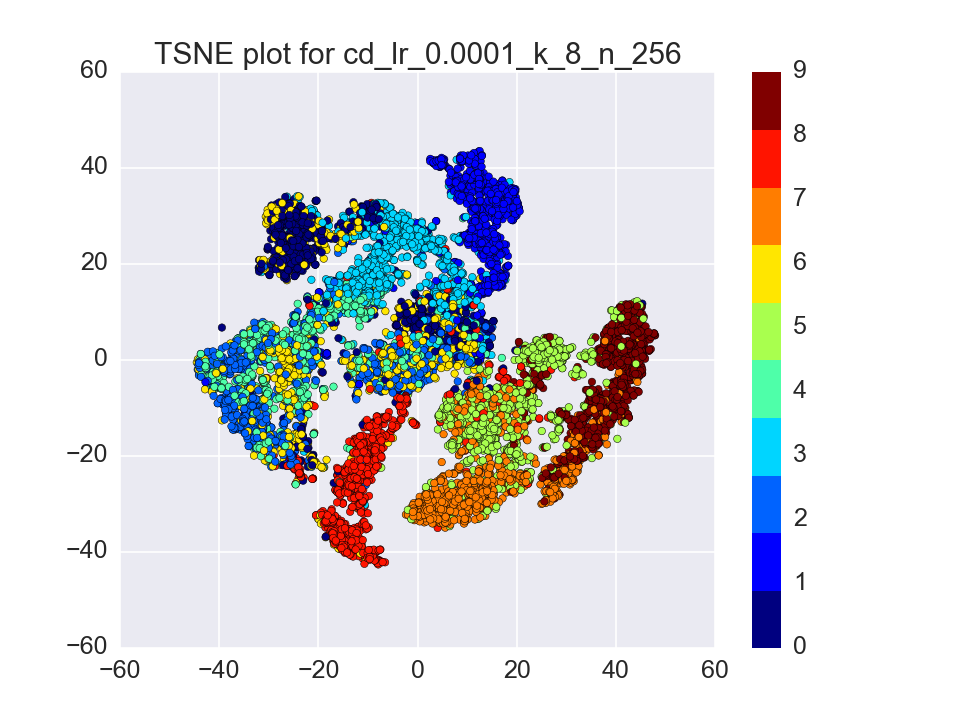
\includegraphics[scale=0.25]{cd_lr_0_0001_k_8_n_256.png}
      %\includegraphics[width=\linewidth, height=60mm]{tiger}
    \end{minipage}
    \\ \hline
    1e-3 & 64 & 16 &
    \begin{minipage}{.3\textwidth}
      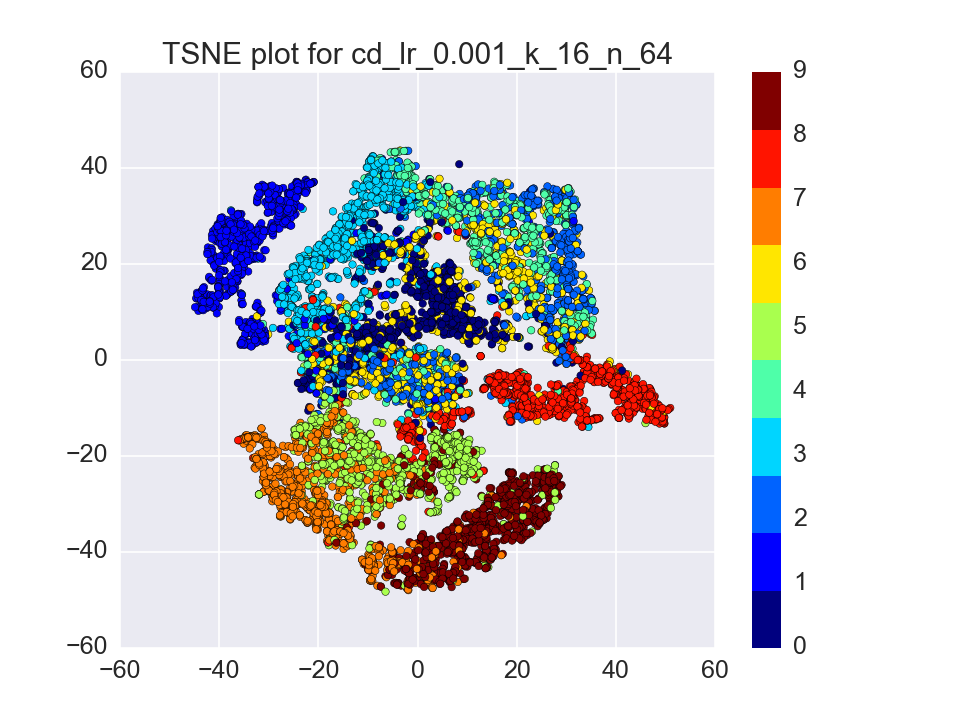
\includegraphics[scale=0.25]{cd_lr_0_001_k_16_n_64.png}
    \end{minipage}
	&
    1e-4 & 256 & 16 &
    \begin{minipage}{.3\textwidth}
      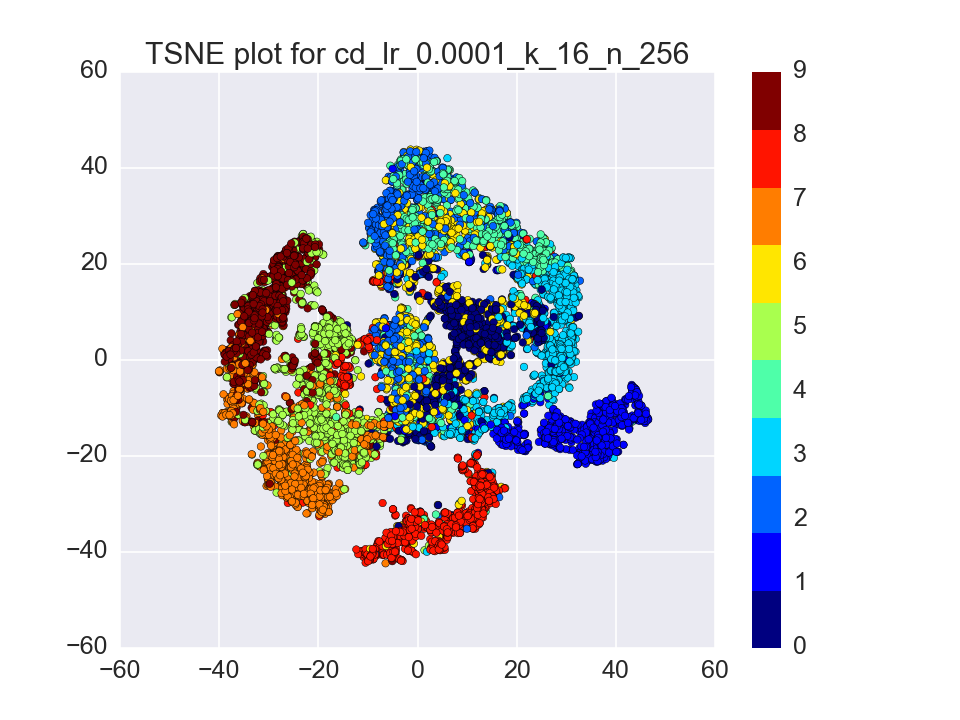
\includegraphics[scale=0.25]{cd_lr_0_0001_k_16_n_256.png}
      %\includegraphics[width=\linewidth, height=60mm]{tiger}
    \end{minipage}
    \\ \hline
    1e-3 & 64 & 32 &
    \begin{minipage}{.3\textwidth}
      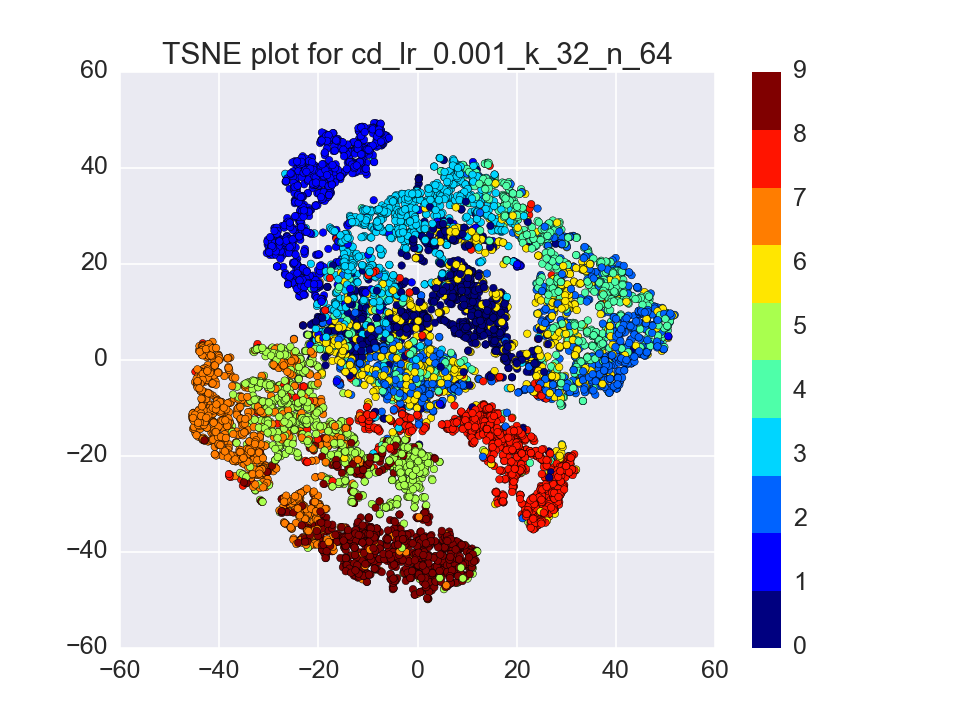
\includegraphics[scale=0.25]{cd_lr_0_001_k_32_n_64.png}
    \end{minipage}
	&
    1e-4 & 256 & 32 &
    \begin{minipage}{.3\textwidth}
      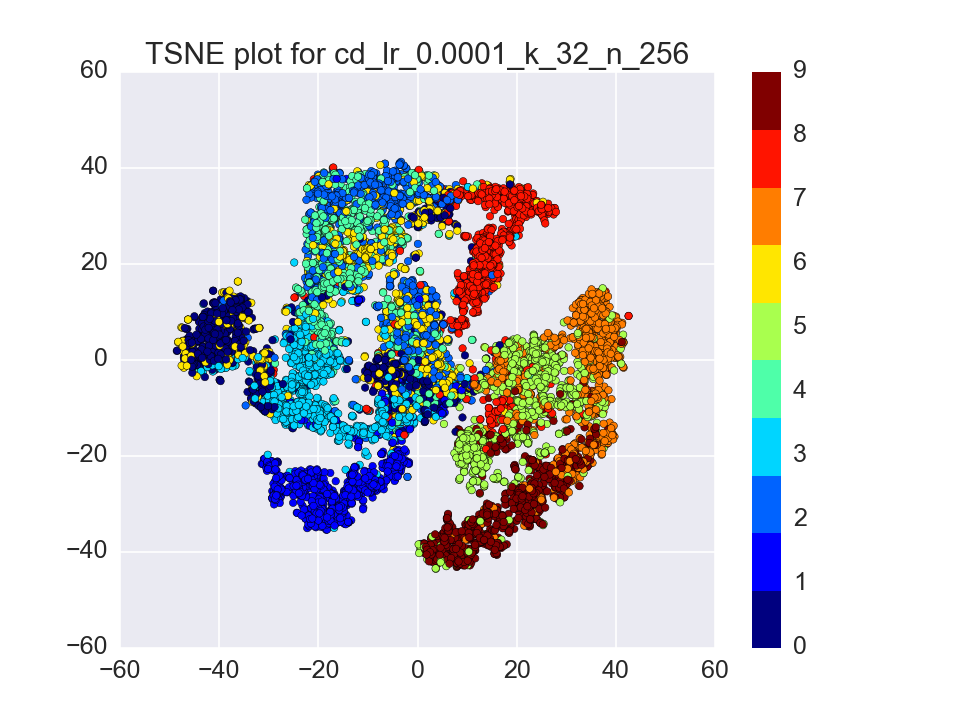
\includegraphics[scale=0.25]{cd_lr_0_0001_k_32_n_256.png}
      %\includegraphics[width=\linewidth, height=60mm]{tiger}
    \end{minipage}
    \\ \hline
  \end{tabular}
\end{table}

\begin{table}[H]
  \centering
  \begin{tabular}{ | c | c | c | c || c | c | c| c |}
    \hline
    \textbf{lr} & \textbf{n} & \textbf{k} & \textbf{t-SNE} & \textbf{lr} & \textbf{n} & \textbf{k} & \textbf{t-SNE} \\
     &  &  &  & & & & \\ \hline
    1e-4 & 128 & 1 &
    \begin{minipage}{.3\textwidth}
      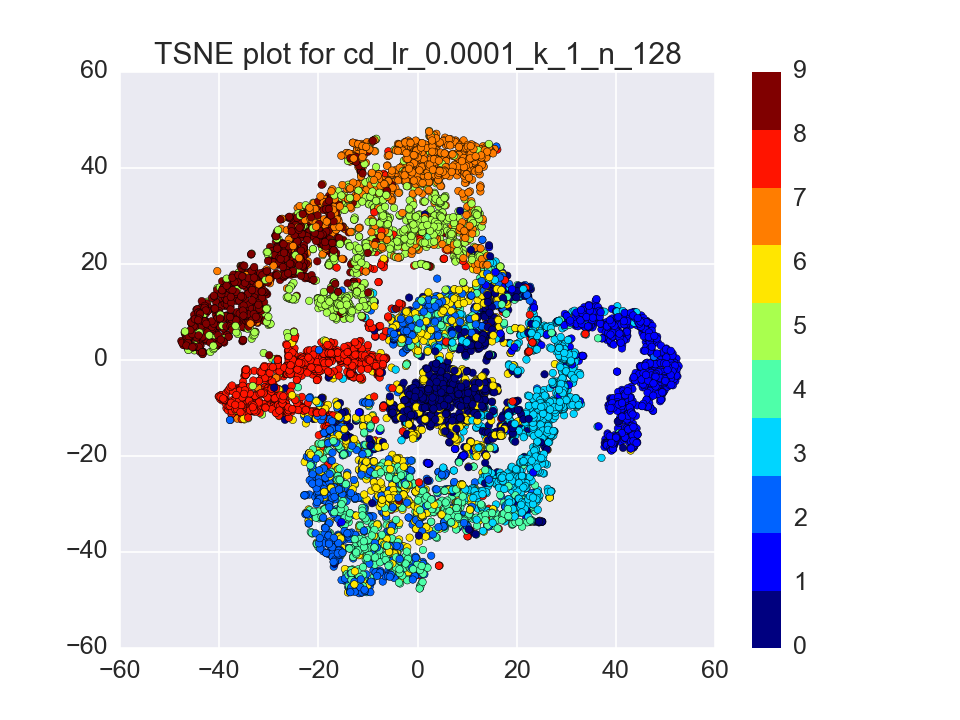
\includegraphics[scale=0.25]{cd_lr_0_0001_k_1_n_128.png}
    \end{minipage}
	&
    1e-4 & 64 & 1 &
    \begin{minipage}{.3\textwidth}
      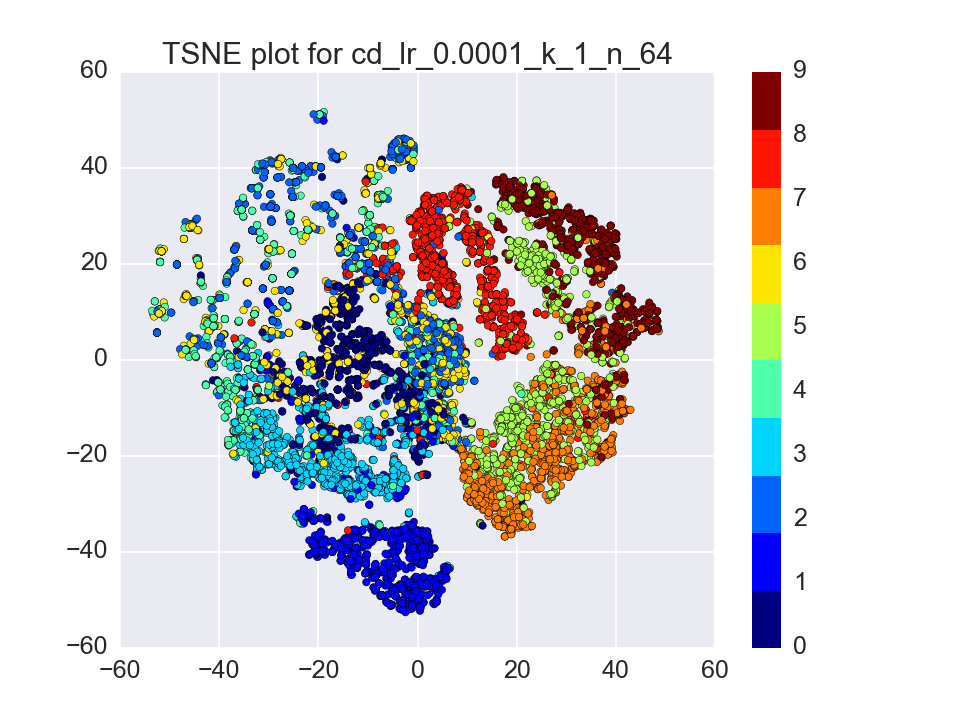
\includegraphics[scale=0.25]{cd_lr_0_0001_k_1_n_64.png}
      %\includegraphics[width=\linewidth, height=60mm]{tiger}
    \end{minipage}
    \\ \hline
    1e-4 & 128 & 2 &
    \begin{minipage}{.3\textwidth}
      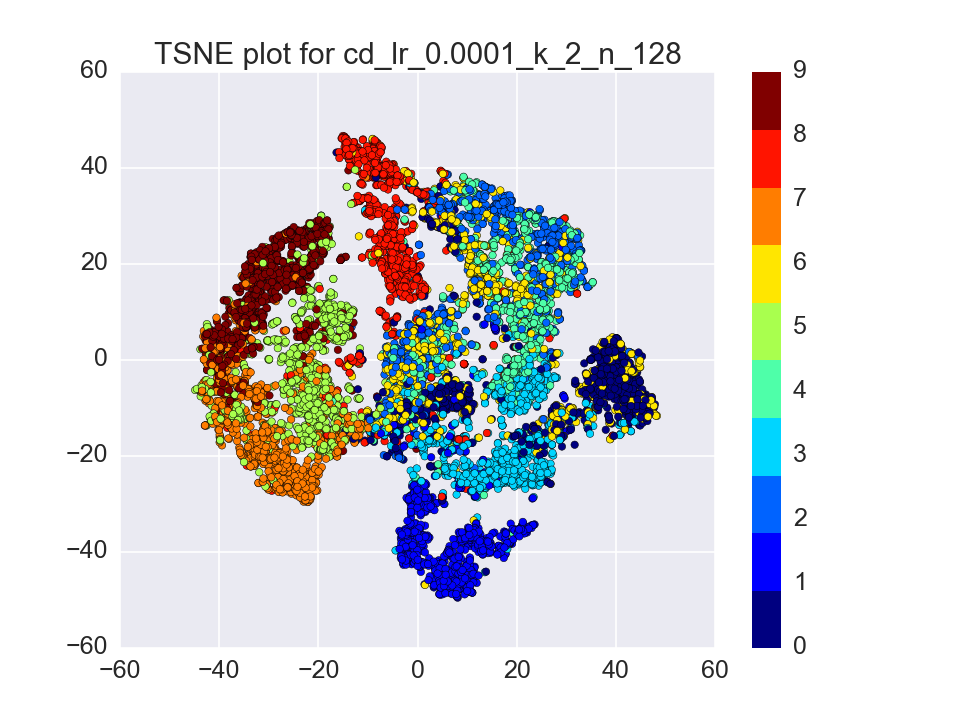
\includegraphics[scale=0.25]{cd_lr_0_0001_k_2_n_128.png}
    \end{minipage}
	&
    1e-4 & 64 & 2 &
    \begin{minipage}{.3\textwidth}
      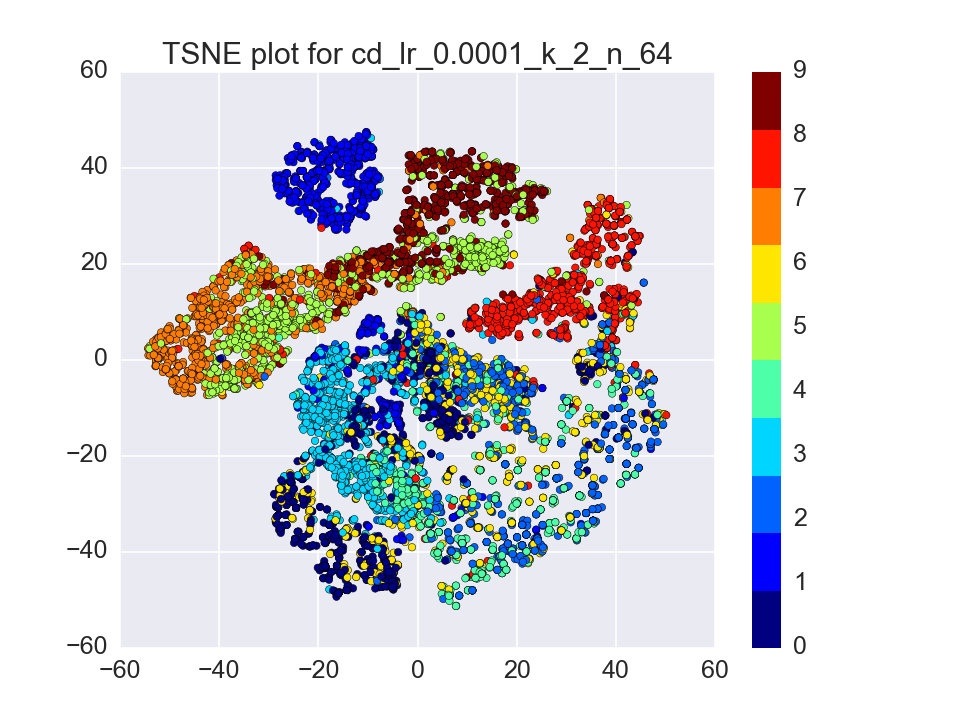
\includegraphics[scale=0.25]{cd_lr_0_0001_k_2_n_64.png}
      %\includegraphics[width=\linewidth, height=60mm]{tiger}
    \end{minipage}
    \\ \hline
    1e-4 & 128 & 4 &
    \begin{minipage}{.3\textwidth}
      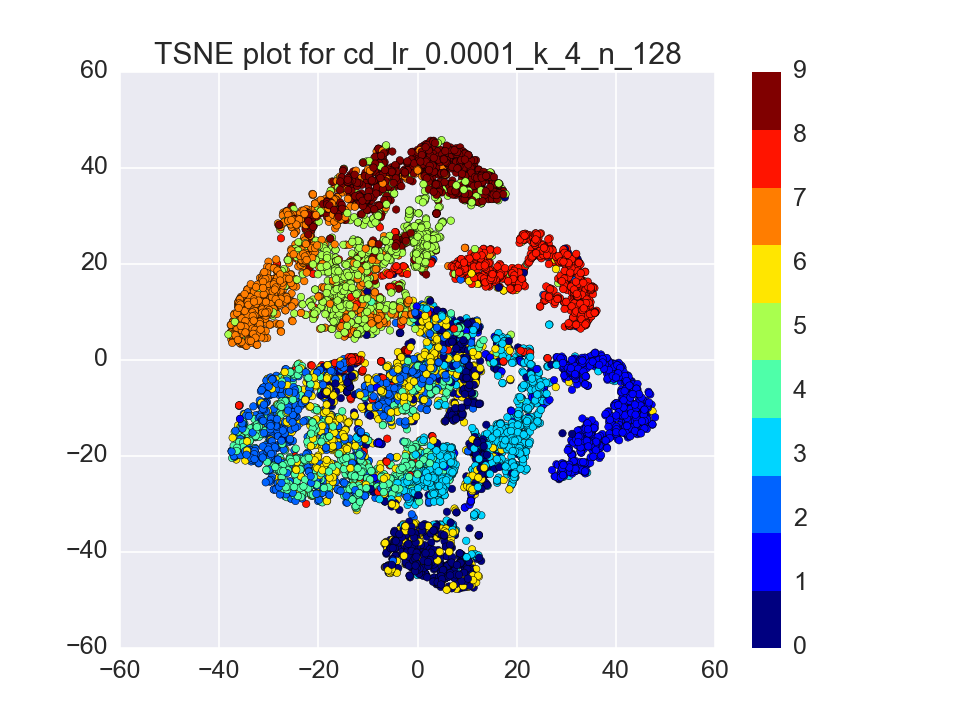
\includegraphics[scale=0.25]{cd_lr_0_0001_k_4_n_128.png}
    \end{minipage}
	&
    1e-4 & 64 & 4 &
    \begin{minipage}{.3\textwidth}
      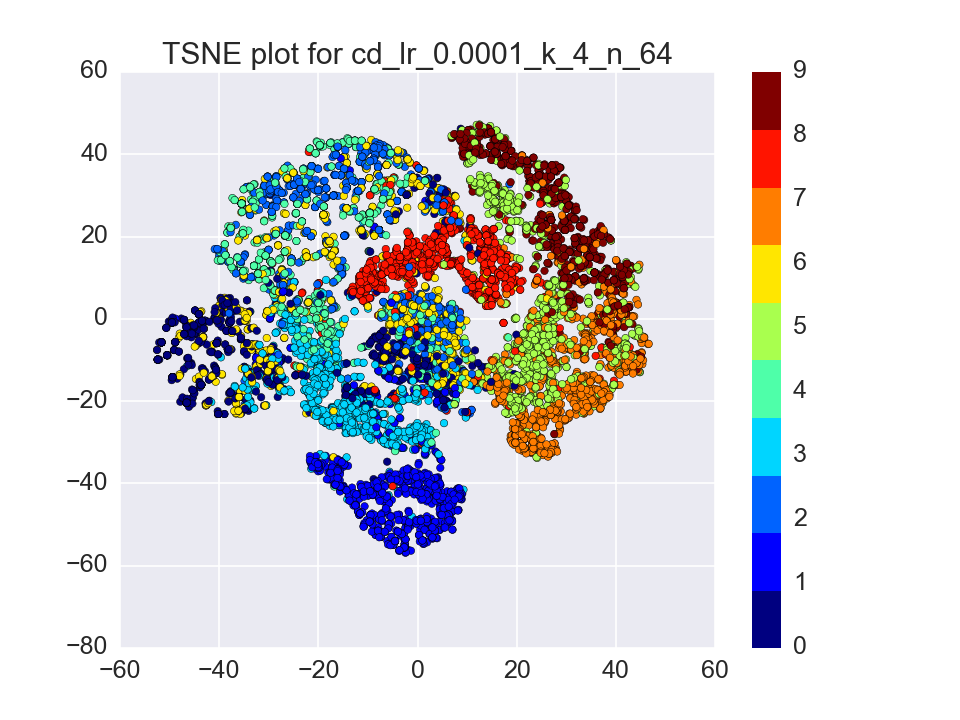
\includegraphics[scale=0.25]{cd_lr_0_0001_k_4_n_64.png}
      %\includegraphics[width=\linewidth, height=60mm]{tiger}
    \end{minipage}
    \\ \hline
        1e-4 & 128 & 8 &
    \begin{minipage}{.3\textwidth}
      \includegraphics[scale=0.25]{cd_lr_0_0001_k_8_n_128.png}
    \end{minipage}
	&
    1e-4 & 64 & 8 &
    \begin{minipage}{.3\textwidth}
      \includegraphics[scale=0.25]{cd_lr_0_0001_k_8_n_64.png}
      %\includegraphics[width=\linewidth, height=60mm]{tiger}
    \end{minipage}
    \\ \hline
        1e-4 & 128 & 16 &
    \begin{minipage}{.3\textwidth}
      \includegraphics[scale=0.25]{cd_lr_0_0001_k_16_n_128.png}
    \end{minipage}
	&
    1e-4 & 64 & 16 &
    \begin{minipage}{.3\textwidth}
      \includegraphics[scale=0.25]{cd_lr_0_0001_k_16_n_64.png}
      %\includegraphics[width=\linewidth, height=60mm]{tiger}
    \end{minipage}
    \\ \hline
        1e-4 & 128 & 32 &
    \begin{minipage}{.3\textwidth}
      \includegraphics[scale=0.25]{cd_lr_0_0001_k_32_n_128.png}
    \end{minipage}
	&
    1e-4 & 64 & 32 &
    \begin{minipage}{.3\textwidth}
      \includegraphics[scale=0.25]{cd_lr_0_0001_k_32_n_64.png}
      %\includegraphics[width=\linewidth, height=60mm]{tiger}
    \end{minipage}
    \\ \hline
  \end{tabular}
\end{table}
%-------------------------------------------------------------------------------
% Question 2
%-------------------------------------------------------------------------------
\section{Effects of k on Gibbs Chain}
\begin{table}[H]
  \centering
  \begin{tabular}{ | c | c | c | c |}
    \hline
    \textbf{lr} & \textbf{n} & \textbf{Train Plot} & \textbf{Test Plot} \\ \hline
    1e-3 & 256 &
    \begin{minipage}{.3\textwidth}
    \includegraphics[scale=0.25]{train_cd_lr_0_001_n_256.png}
    \end{minipage} &
    \begin{minipage}{.3\textwidth}
      \includegraphics[scale=0.25]{cd_lr_0_001_n_256.png}
    \end{minipage}
    \\ \hline
    1e-3 & 128 &
    \begin{minipage}{.3\textwidth}
    \includegraphics[scale=0.25]{train_cd_lr_0_001_n_128.png}
    \end{minipage} &
    \begin{minipage}{.3\textwidth}
      \includegraphics[scale=0.25]{cd_lr_0_001_n_128.png}
    \end{minipage}
    \\ \hline
    1e-3 & 64 &
    \begin{minipage}{.3\textwidth}
      \includegraphics[scale=0.25]{train_cd_lr_0_001_n_64.png}
    \end{minipage} &
    \begin{minipage}{.3\textwidth}
      \includegraphics[scale=0.25]{cd_lr_0_001_n_64.png}
    \end{minipage}
    \\ \hline
  \end{tabular}
\end{table}

\section{Effects of k on Gibbs Chain}
\begin{table}[H]
  \centering
  \begin{tabular}{ | c | c | c | c |}
    \hline
    \textbf{lr} & \textbf{n} & \textbf{Train Plot} & \textbf{Test Plot} \\ \hline
    1e-4 & 256 &
    \begin{minipage}{.3\textwidth}
      \includegraphics[scale=0.25]{train_cd_lr_0_0001_n_256.png}
    \end{minipage} &
    \begin{minipage}{.3\textwidth}
      \includegraphics[scale=0.25]{cd_lr_0_0001_n_256.png}
    \end{minipage}
    \\ \hline
    1e-4 & 128 &
    \begin{minipage}{.3\textwidth}
      \includegraphics[scale=0.25]{train_cd_lr_0_0001_n_128.png}
    \end{minipage} &
    \begin{minipage}{.3\textwidth}
      \includegraphics[scale=0.25]{cd_lr_0_0001_n_128.png}
    \end{minipage}
    \\ \hline
    1e-4 & 64 &
    \begin{minipage}{.3\textwidth}
      \includegraphics[scale=0.25]{train_cd_lr_0_0001_n_64.png}
    \end{minipage} &
    \begin{minipage}{.3\textwidth}
      \includegraphics[scale=0.25]{cd_lr_0_0001_n_64.png}
    \end{minipage}
    \\ \hline
  \end{tabular}
\end{table}

\section{Effects of k on Gibbs Chain}
\begin{table}[H]
  \centering
  \begin{tabular}{ | c | c | c | c |}
    \hline
    \textbf{lr} & \textbf{n} & \textbf{Train Plot} & \textbf{Test Plot} \\ \hline
    1e-5 & 256 &
    \begin{minipage}{.3\textwidth}
      \includegraphics[scale=0.25]{train_cd_lr_0_00001_n_256.png}
    \end{minipage} &
    \begin{minipage}{.3\textwidth}
      \includegraphics[scale=0.25]{cd_lr_0_00001_n_256.png}
    \end{minipage}
    \\ \hline
    1e-5 & 128 &
    \begin{minipage}{.3\textwidth}
      \includegraphics[scale=0.25]{train_cd_lr_0_00001_n_128.png}
    \end{minipage} &
    \begin{minipage}{.3\textwidth}
      \includegraphics[scale=0.25]{cd_lr_0_00001_n_128.png}
    \end{minipage}
    \\ \hline
    1e-5 & 64 &
    \begin{minipage}{.3\textwidth}
      \includegraphics[scale=0.25]{train_cd_lr_0_00001_n_64.png}
    \end{minipage} &
    \begin{minipage}{.3\textwidth}
      \includegraphics[scale=0.25]{cd_lr_0_00001_n_64.png}
    \end{minipage}
    \\ \hline
  \end{tabular}
\end{table}
%-------------------------------------------------------------------------------
% Question 3
%-------------------------------------------------------------------------------
\section{Plots of samples generated by Gibbs Chain}
\section{Effects of k on Gibbs Chain}
\begin{table}[H]
  \centering
  \begin{tabular}{ | c | c | c | c | c | c |}
    \hline
    \textbf{Original} & \textbf{1 epoch} & \textbf{2 epoch} & \textbf{4 epoch} & \textbf{16 epoch}  & \textbf{40 epoch} \\ \hline
    \begin{minipage}{.3\textwidth}
      \includegraphics[scale=0.2]{BM_avisual.png}
    \end{minipage} & 
    \begin{minipage}{.3\textwidth}
      \includegraphics[scale=0.2]{BM_a1.png}
    \end{minipage} &
    \begin{minipage}{.3\textwidth}
      \includegraphics[scale=0.2]{BM_a2.png}
    \end{minipage} &
    \begin{minipage}{.3\textwidth}
      \includegraphics[scale=0.2]{BM_a4.png}
    \end{minipage} &
    \begin{minipage}{.3\textwidth}
      \includegraphics[scale=0.2]{BM_a16.png}
    \end{minipage} &
    \begin{minipage}{.3\textwidth}
      \includegraphics[scale=0.2]{BM_a40.png}
    \end{minipage}
    \\ \hline
  \end{tabular}
\end{table}

%-------------------------------------------------------------------------------
% Question 4
%-------------------------------------------------------------------------------
\section{Gibbs Sampling}


%-------------------------------------------------------------------------------
% REFERENCES
%-------------------------------------------------------------------------------
\begin{thebibliography}{9}
\bibitem{1} 
Mitesh M Khapra. \textit{CS7015 Deep Learning: Lecture 13-18}, 
Indian Institute of Technology Madras, 2018
\end{thebibliography}


\end{document}

%-------------------------------------------------------------------------------
% SNIPPETS
%-------------------------------------------------------------------------------

%\begin{figure}[!ht]
%	\centering
%	\includegraphics[width=0.8\textwidth]{file_name}
%	\caption{}
%	\centering
%	\label{label:file_name}
%\end{figure}

%\begin{figure}[!ht]
%	\centering
%	\includegraphics[width=0.8\textwidth]{graph}
%	\caption{Blood pressure ranges and associated level of hypertension (American Heart Association, 2013).}
%	\centering
%	\label{label:graph}
%\end{figure}

%\begin{wrapfigure}{r}{0.30\textwidth}
%	\vspace{-40pt}
%	\begin{center}
%		\includegraphics[width=0.29\textwidth]{file_name}
%	\end{center}
%	\vspace{-20pt}
%	\caption{}
%	\label{label:file_name}
%\end{wrapfigure}

%\begin{wrapfigure}{r}{0.45\textwidth}
%	\begin{center}
%		\includegraphics[width=0.29\textwidth]{manometer}
%	\end{center}
%	\caption{Aneroid sphygmomanometer with stethoscope (Medicalexpo, 2012).}
%	\label{label:manometer}
%\end{wrapfigure}

%\begin{table}[!ht]\footnotesize
%	\centering
%	\begin{tabular}{cccccc}
%	\toprule
%	\multicolumn{2}{c} {Pearson's correlation test} & \multicolumn{4}{c} {Independent t-test} \\
%	\midrule	
%	\multicolumn{2}{c} {Gender} & \multicolumn{2}{c} {Activity level} & \multicolumn{2}{c} {Gender} \\
%	\midrule
%	Males & Females & 1st level & 6th level & Males & Females \\
%	\midrule
%	\multicolumn{2}{c} {BMI vs. SP} & \multicolumn{2}{c} {Systolic pressure} & \multicolumn{2}{c} {Systolic Pressure} \\
%	\multicolumn{2}{c} {BMI vs. DP} & \multicolumn{2}{c} {Diastolic pressure} & \multicolumn{2}{c} {Diastolic pressure} \\
%	\multicolumn{2}{c} {BMI vs. MAP} & \multicolumn{2}{c} {MAP} & \multicolumn{2}{c} {MAP} \\
%	\multicolumn{2}{c} {W:H ratio vs. SP} & \multicolumn{2}{c} {BMI} & \multicolumn{2}{c} {BMI} \\
%	\multicolumn{2}{c} {W:H ratio vs. DP} & \multicolumn{2}{c} {W:H ratio} & \multicolumn{2}{c} {W:H ratio} \\
%	\multicolumn{2}{c} {W:H ratio vs. MAP} & \multicolumn{2}{c} {\% Body fat} & \multicolumn{2}{c} {\% Body fat} \\
%	\multicolumn{2}{c} {} & \multicolumn{2}{c} {Height} & \multicolumn{2}{c} {Height} \\
%	\multicolumn{2}{c} {} & \multicolumn{2}{c} {Weight} & \multicolumn{2}{c} {Weight} \\
%	\multicolumn{2}{c} {} & \multicolumn{2}{c} {Heart rate} & \multicolumn{2}{c} {Heart rate} \\
%	\bottomrule
%	\end{tabular}
%	\caption{Parameters that were analysed and related statistical test performed for current study. BMI - body mass index; SP - systolic pressure; DP - diastolic pressure; MAP - mean arterial pressure; W:H ratio - waist to hip ratio.}
%	\label{label:tests}
%\end{table}